\subsection{Additional Figure(s) and Table(s)}
% 1. Figure(s)
% \afterpage{
    \begin{figure}[ht!]
        \centering
        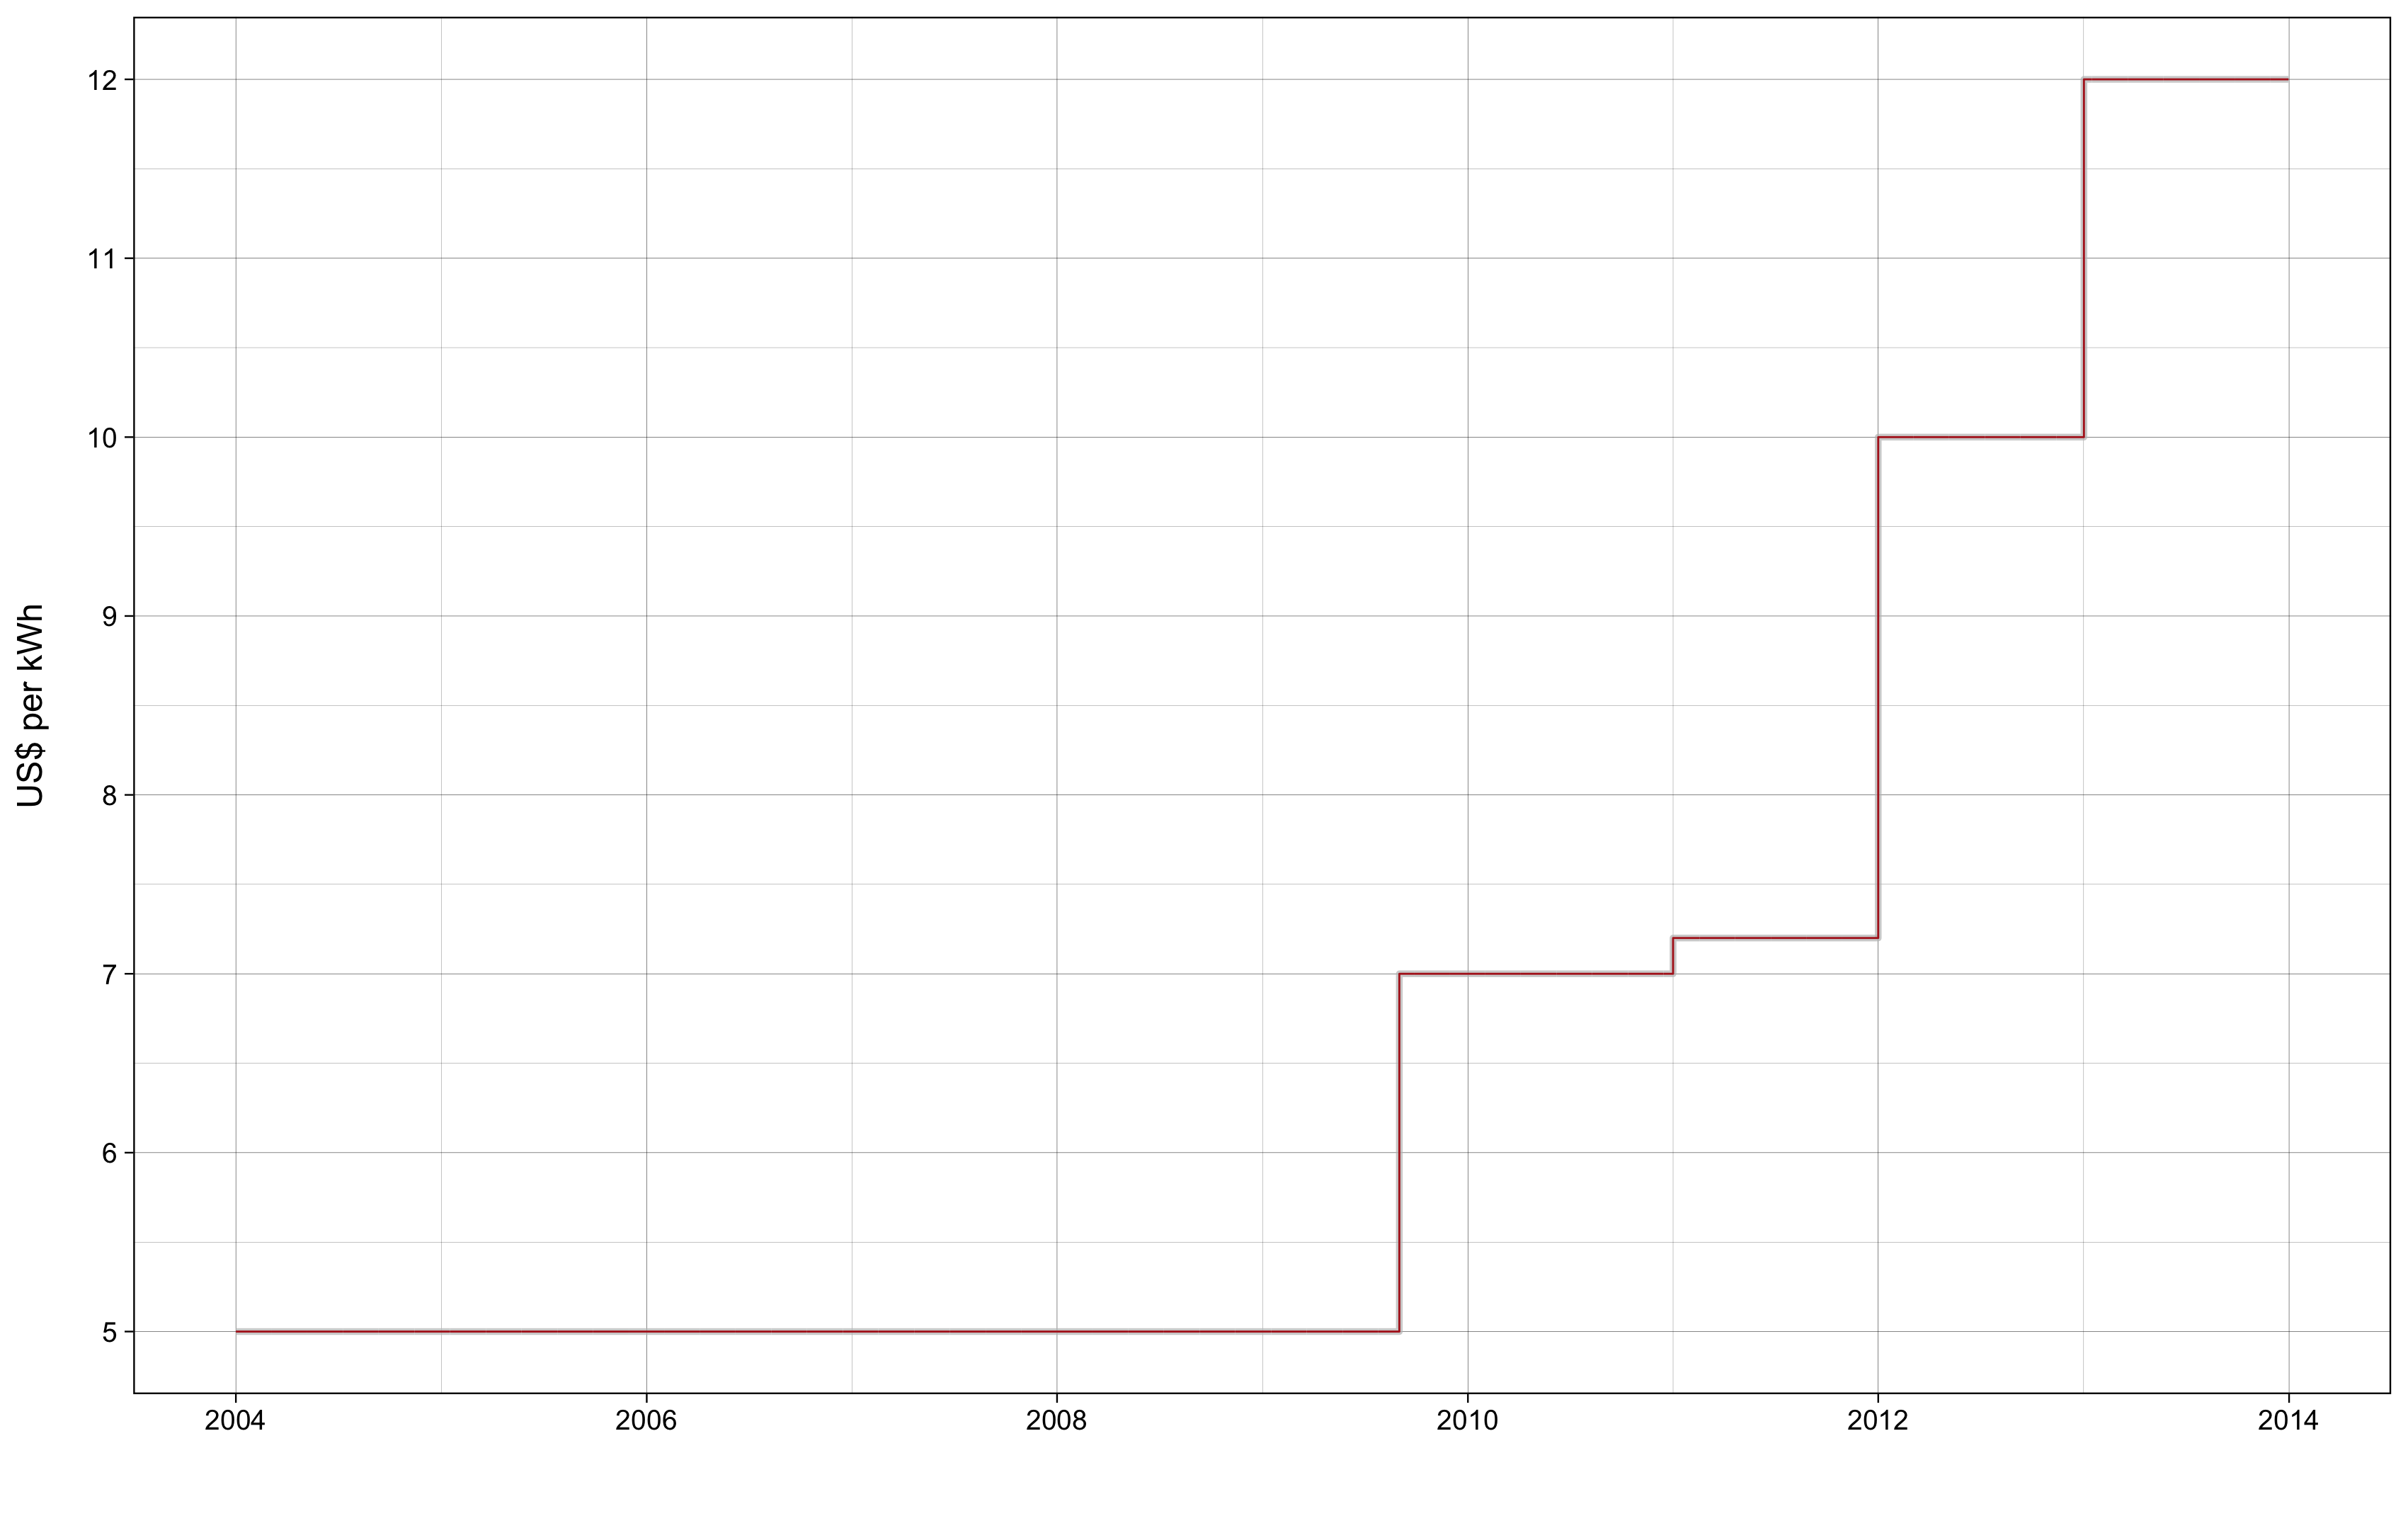
\includegraphics[scale = 0.133]{02_Chapter-1/00A_Figures/Figure_SMUD-Residential-Rates_Fixed-Charge.png}
        \caption{Fixed Charge of SMUD Residential Rates}
        \caption*{
            {\small
            \textit{Note}: 
            The figure shows how SMUD changed the monthly fixed charge over time. The same fixed charge applies to households that choose one of the three major residential rate plans (i.e., RSCH, RSEH, and RSGH).
        }}
        \label{Figure:SMUD-Residential-Rates_Fixed-Charge}
    \end{figure}
% }

\afterpage{
    \begin{figure}[t!]
        \centering
        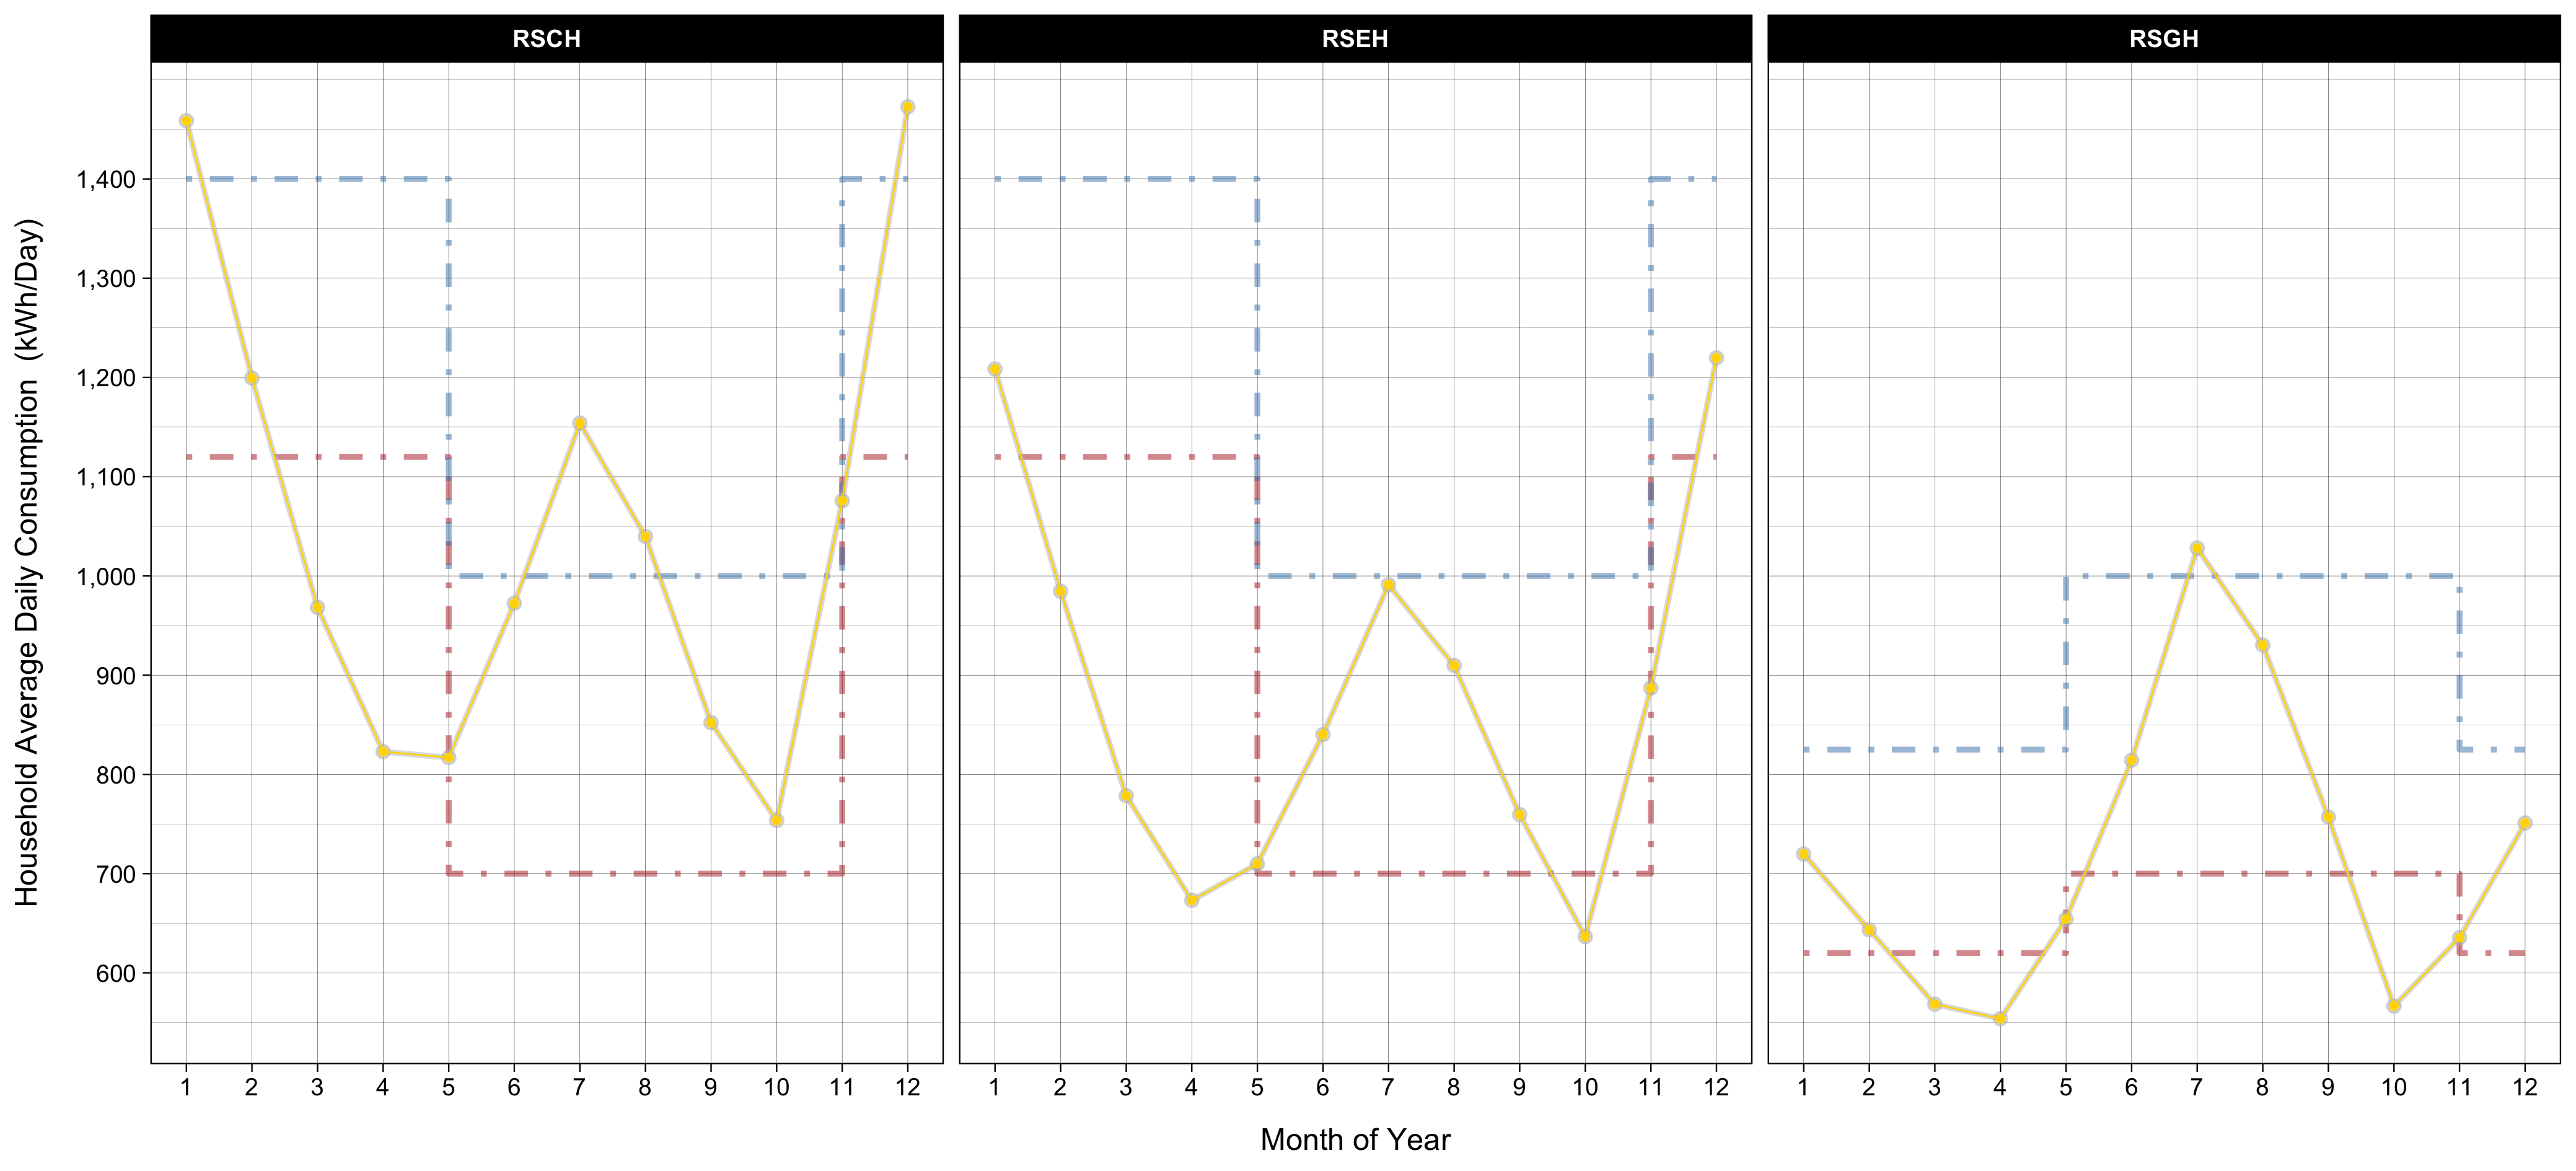
\includegraphics[scale = 0.105]{02_Chapter-1/00A_Figures/Figure_Household-Average-Daily-Consumption-by-Month.png}
        \caption{Household Average Daily Electricity Consumption by Month of Year}
        \caption*{
            {\small
            \textit{Note}: 
            This figure depicts, for each of SMUD residential rate plans, how households' average daily electricity consumption varied across months of the year. The red and blue dot-dash lines represent the lower and higher base usage quantities in each month of the year, respectively. The three rate plans show similar consumption and seasonal patterns. 
        }}
        \label{Figure:Household-Average-Daily-Electricity-Consumption-by-Month-of-Year}
    \end{figure}
}
\clearpage

% \afterpage{
    \begin{figure}[ht!]
        \centering
        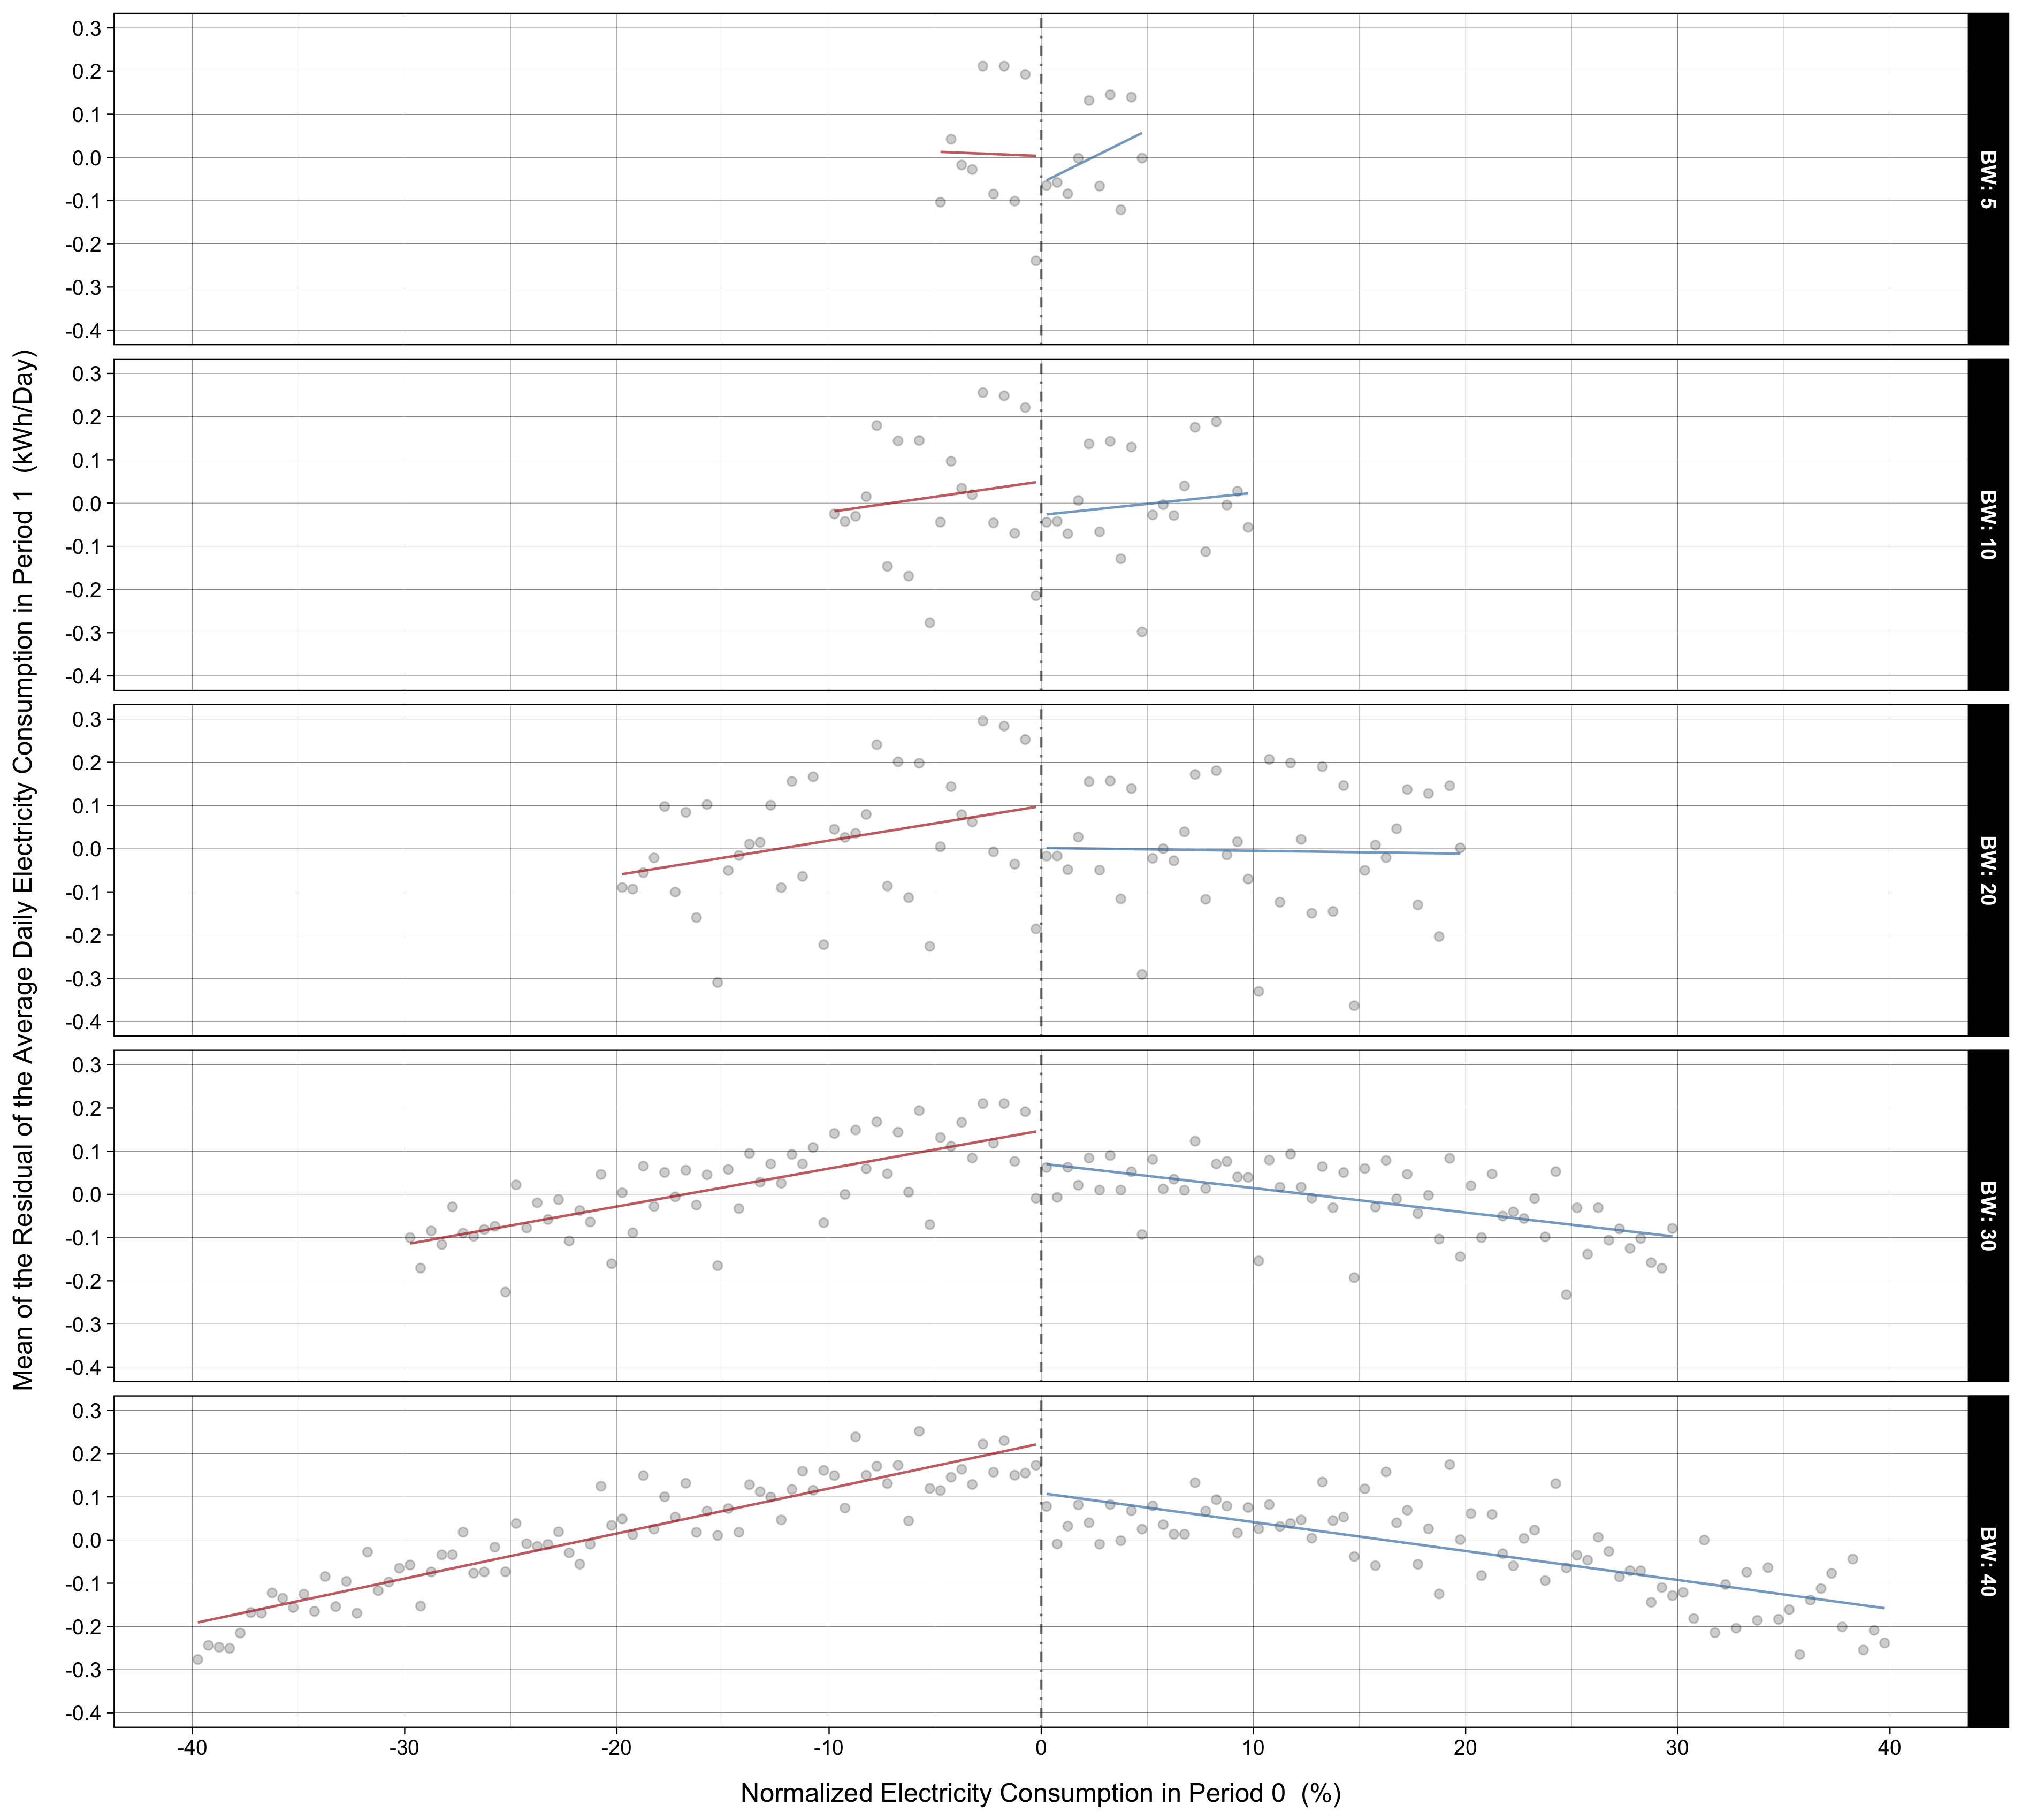
\includegraphics[scale = 0.120]{02_Chapter-1/00A_Figures/Figure_Residuals-of-the-Average-Daily-Electricity-Consumption-in-Period-0-over-NC0_From-BW5-to-BW40.png}
        \caption{The Impact of the Change in the Marginal Price due to Surpassing the Lower Base Usage Quantity}
        \caption*{
            {\small
            \textit{Note}: 
            In this figure, scatter dots correspond to the mean of residuals, computed by bins with a bandwidth of 0.5\%, from a regression of households' average daily electricity consumption in Period 1 on $\widebar{NC}_{0}$, HDDs and CDDs. As described, a linear model fits those scatter points well, even for a wide bandwidth. 
        }}
        \label{Figure:The-Impact-of-the-Change-in-the-MP-due-to-Surpassing-the-Lower-BUQ}
    \end{figure}
% }
\clearpage



% 2. Table(s)
\afterpage{
    \begin{table}[t!]
        \centering
        \caption{Robustness Checks: For Different Functional Forms, 3rd- and 4th-Order Polynomial Models}
        \label{Table:Robustness-Checks_Functional-Forms_3rd-and-4th-Order-Polynomial-Models}
        \vspace{0.3cm}
        \footnotesize
        \begin{adjustbox}{scale = 0.9}
            \begin{threeparttable}
                \begin{tabular}{@{\extracolsep{3pt}}lcccccccc}
                    \\[-5.5ex]
                    \hline \hline
                    \\[-3.0ex]
                     & \multicolumn{8}{c}{Dependent Variable} \\
                    \\[-3.0ex]
                    \cline{2-9}
                    \\[-3.0ex]
                     & \multicolumn{8}{c}{Average Daily Electricity Consumption  (kWh/Day)} \\
                    \\[-3.0ex]
                     & (1) & (2) & (3) & (4) & (5) & (6) & (7) & (8) \\
                    \\[-3.0ex]
                    \hline
                    \\[-2.0ex]
                    $\mathbb{1}$[Treatment] & 0.049 & $-$0.022 & $-$0.056$^{***}$ & $-$0.101$^{***}$ & 0.129$^{**}$ & 0.019 & $-$0.049$^{**}$ & $-$0.068$^{**}$ \\ 
                    & (0.042) & (0.025) & (0.017) & (0.028) & (0.051) & (0.037) & (0.021) & (0.027) \\ 
                    & & & & & & & & \\ 
                    NC0 & 0.143$^{***}$ & 0.211$^{***}$ & 0.215$^{***}$ & 0.225$^{***}$ & 0.111$^{**}$ & 0.207$^{***}$ & 0.213$^{***}$ & 0.217$^{***}$ \\ 
                    & (0.022) & (0.010) & (0.006) & (0.010) & (0.043) & (0.016) & (0.008) & (0.011) \\ 
                    & & & & & & & & \\ 
                    $\mathbb{1}$[Treatment] $\times$ NC0 & 0.056 & 0.005 & $-$0.007 & 0.0003 & $-$0.035 & $-$0.027 & $-$0.008 & $-$0.001 \\ 
                    & (0.035) & (0.013) & (0.005) & (0.005) & (0.079) & (0.021) & (0.008) & (0.010) \\ 
                    & & & & & & & & \\ 
                    NC0$^{2}$ & $-$0.020$^{***}$ & $-$0.002 & $-$0.0003 & $-$0.0001 & $-$0.035$^{**}$ & $-$0.003 & $-$0.001 & $-$0.001$^{*}$ \\ 
                    & (0.005) & (0.001) & (0.0002) & (0.0002) & (0.017) & (0.003) & (0.001) & (0.001) \\ 
                    & & & & & & & & \\ 
                    $\mathbb{1}$[Treatment] $\times$ NC0$^{2}$ & 0.022$^{***}$ & 0.001 & 0.0004 & $-$0.0004 & 0.092$^{***}$ & 0.010$^{**}$ & 0.001 & 0.001$^{**}$ \\ 
                    & (0.008) & (0.001) & (0.0003) & (0.0003) & (0.024) & (0.005) & (0.001) & (0.001) \\ 
                    & & & & & & & & \\ 
                    NC0$^{3}$ & $-$0.001$^{***}$ & $-$0.00005 & $-$0.00000 & 0.00000 & $-$0.004 & $-$0.0001 & $-$0.00002 & $-$0.00003$^{*}$ \\ 
                    & (0.0003) & (0.00003) & (0.00001) & (0.00000) & (0.002) & (0.0002) & (0.00004) & (0.00002) \\ 
                    & & & & & & & & \\ 
                    $\mathbb{1}$[Treatment] $\times$ NC0$^{3}$ & 0.001$^{**}$ & 0.0001 & $-$0.00000 & 0.00000 & $-$0.005 & $-$0.0005$^{*}$ & $-$0.00001 & $-$0.00000 \\ 
                    & (0.001) & (0.00005) & (0.00001) & (0.00001) & (0.005) & (0.0003) & (0.0001) & (0.00004) \\ 
                    & & & & & & & & \\ 
                    NC0$^{4}$ &  &  &  &  & $-$0.0001 & $-$0.00000 & $-$0.00000 & $-$0.00000$^{*}$ \\ 
                    &  &  &  &  & (0.0001) & (0.00000) & (0.00000) & (0.00000) \\ 
                    & & & & & & & & \\ 
                    $\mathbb{1}$[Treatment] $\times$ NC0$^{4}$ &  &  &  &  & 0.001$^{***}$ & 0.00002$^{*}$ & 0.00000 & 0.00000$^{**}$ \\ 
                    &  &  &  &  & (0.0002) & (0.00001) & (0.00000) & (0.00000) \\ 
                    & & & & & & & & \\ 
                    Average Daily CDDs & 1.146$^{***}$ & 1.146$^{***}$ & 1.135$^{***}$ & 1.133$^{***}$ & 1.146$^{***}$ & 1.146$^{***}$ & 1.135$^{***}$ & 1.133$^{***}$ \\ 
                    & (0.106) & (0.105) & (0.109) & (0.129) & (0.106) & (0.105) & (0.109) & (0.129) \\ 
                    & & & & & & & & \\ 
                    Average Daily HDDs & 0.428$^{***}$ & 0.431$^{***}$ & 0.375$^{***}$ & 0.742$^{***}$ & 0.428$^{***}$ & 0.431$^{***}$ & 0.375$^{***}$ & 0.742$^{***}$ \\ 
                    & (0.106) & (0.104) & (0.128) & (0.202) & (0.106) & (0.104) & (0.128) & (0.202) \\ 
                    & & & & & & & & \\
                    \hline
                    \\[-2.0ex]
                    Bandwidth & 10\% & 20\% & 30\% & 40\% & 10\% & 20\% & 30\% & 40\% \\ 
                    FEs: Billing Year-by-Month & Yes & Yes & Yes & Yes & Yes & Yes & Yes & Yes \\ 
                    Observations & 2,378,864 & 4,702,081 & 6,276,579 & 3,904,120 & 2,378,864 & 4,702,081 & 6,276,579 & 3,904,120 \\ 
                    Adjusted R$^{2}$ & 0.293 & 0.334 & 0.536 & 0.592 & 0.293 & 0.334 & 0.536 & 0.592 \\
                    \\[-2.0ex]
                    \hline \hline
                    \\[-4.5ex]
                \end{tabular}
                \begin{tablenotes}[flushleft]
                    \footnotesize
                    \item \textit{Note}: * $p < 0.1$, ** $p < 0.05$, and *** $p < 0.01$.
                \end{tablenotes}
            \end{threeparttable}
        \end{adjustbox}
        
    \end{table}
}

\clearpage

\afterpage{
    \begin{table}[t!]
        \centering
        \caption{Robustness Checks: For Different Bandwidths, Without FEs}
        \label{Table:Robustness-Checks_BWs_Without-FEs}
        \vspace{0.3cm}
        \footnotesize
        \begin{adjustbox}{scale = 0.76}
            \begin{threeparttable}
                \begin{tabular}{@{\extracolsep{5pt}}lcccccccc}
                    \\[-5.5ex]
                    \hline \hline
                    \\[-3.0ex]
                     & \multicolumn{8}{c}{Dependent Variable} \\
                    \\[-3.0ex]
                    \cline{2-9}
                    \\[-3.0ex]
                     & \multicolumn{8}{c}{Average Daily Electricity Consumption  (kWh/Day)} \\
                    \\[-3.0ex]
                     & (1) & (2) & (3) & (4) & (5) & (6) & (7) & (8) \\
                    \\[-3.0ex]
                    \hline
                    \\[-2.0ex]
                    $\mathbb{1}$[Treatment] & $-$0.014 & $-$0.054$^{*}$ & $-$0.053$^{*}$ & $-$0.084$^{***}$ & $-$0.076$^{***}$ & $-$0.072$^{**}$ & $-$0.097$^{*}$ & $-$0.118$^{*}$ \\ 
                    & (0.032) & (0.030) & (0.028) & (0.028) & (0.029) & (0.031) & (0.056) & (0.064) \\ 
                    & & & & & & & & \\ 
                    NC0 & 0.169$^{***}$ & 0.197$^{***}$ & 0.202$^{***}$ & 0.204$^{***}$ & 0.204$^{***}$ & 0.199$^{***}$ & 0.214$^{***}$ & 0.211$^{***}$ \\ 
                    & (0.010) & (0.007) & (0.006) & (0.006) & (0.006) & (0.006) & (0.009) & (0.009) \\ 
                    & & & & & & & & \\ 
                    $\mathbb{1}$[Treatment] $\times$ NC0 & 0.038$^{***}$ & 0.001 & $-$0.010$^{***}$ & $-$0.008$^{***}$ & $-$0.009$^{***}$ & $-$0.014$^{***}$ & $-$0.018$^{***}$ & $-$0.017$^{***}$ \\ 
                    & (0.012) & (0.004) & (0.003) & (0.003) & (0.003) & (0.003) & (0.004) & (0.005) \\ 
                    & & & & & & & & \\ 
                    Average Daily CDDs & 0.749$^{***}$ & 0.753$^{***}$ & 0.755$^{***}$ & 0.757$^{***}$ & 0.758$^{***}$ & 0.767$^{***}$ & 0.932$^{***}$ & 1.143$^{***}$ \\ 
                    & (0.122) & (0.121) & (0.120) & (0.119) & (0.118) & (0.114) & (0.124) & (0.124) \\ 
                    & & & & & & & & \\ 
                    Average Daily HDDs & 0.280$^{***}$ & 0.281$^{***}$ & 0.282$^{***}$ & 0.284$^{***}$ & 0.286$^{***}$ & 0.152$^{**}$ & 0.637$^{***}$ & 1.033$^{***}$ \\ 
                    & (0.079) & (0.078) & (0.078) & (0.077) & (0.077) & (0.066) & (0.101) & (0.131) \\ 
                    & & & & & & & & \\ 
                    (Constant) & 19.947$^{***}$ & 19.973$^{***}$ & 19.972$^{***}$ & 19.965$^{***}$ & 19.937$^{***}$ & 19.720$^{***}$ & 17.769$^{***}$ & 15.117$^{***}$ \\ 
                    & (0.948) & (0.941) & (0.937) & (0.932) & (0.926) & (0.829) & (1.082) & (1.159) \\ 
                    & & & & & & & & \\
                    \hline
                    \\[-2.0ex]
                    Bandwidth & 5\% & 10\% & 15\% & 20\% & 25\% & 30\% & 35\% & 40\% \\ 
                    FEs: Billing Year-by-Month & No & No & No & No & No & No & No & No \\ 
                    Observations & 1,186,630 & 2,378,864 & 3,566,318 & 4,702,081 & 5,816,854 & 6,276,579 & 4,093,259 & 3,904,120 \\ 
                    Adjusted R$^{2}$ & 0.105 & 0.120 & 0.144 & 0.175 & 0.210 & 0.349 & 0.394 & 0.468 \\
                    \\[-2.0ex]
                    \hline \hline
                    \\[-4.5ex]
                \end{tabular}
                \begin{tablenotes}[flushleft]
                    \footnotesize
                    \item \textit{Note}: Contrary to Table \ref{Table:Robustness-Checks_BWs}, this table reports the results of robustness checks for a range of bandwidths using the regression in the specification (5) in Table \ref{Table:RD-Results}. Standard errors in parentheses are clustered at the household and billing year-by-month levels to allow correlations across households in a given month; * $p < 0.1$, ** $p < 0.05$, and *** $p < 0.01$.
                \end{tablenotes}
            \end{threeparttable}
        \end{adjustbox}
    \end{table}
}

\clearpage

\afterpage{
    \begin{table}[t!]
        \centering
        \caption{Robustness Checks: For Different Bandwidths, Only RSGH Rate Code}
        \label{Table:Robustness-Checks_BWs_RSGH}
        \vspace{0.3cm}
        \small
        \begin{adjustbox}{scale = 0.72}
            \begin{threeparttable}
                \begin{tabular}{@{\extracolsep{5pt}}lcccccccc}
                    \\[-5.5ex]
                    \hline \hline
                    \\[-3.0ex]
                    & \multicolumn{8}{c}{Dependent Variable} \\
                    \\[-3.0ex]
                    \cline{2-9}
                    \\[-3.0ex]
                    & \multicolumn{8}{c}{Average Daily Electricity Consumption  (kWh/Day)} \\
                    \\[-3.0ex]
                    & (1) & (2) & (3) & (4) & (5) & (6) & (7) & (8) \\
                    \\[-3.0ex]
                    \hline
                    \\[-2.0ex]
                    $\mathbb{1}$[Treatment] & $-$0.055$^{***}$ & $-$0.060$^{***}$ & $-$0.055$^{***}$ & $-$0.065$^{***}$ & $-$0.064$^{***}$ & $-$0.058$^{***}$ & $-$0.068$^{***}$ & $-$0.080$^{***}$ \\ 
                    & (0.020) & (0.016) & (0.015) & (0.014) & (0.013) & (0.013) & (0.021) & (0.024) \\ 
                    & & & & & & & & \\ 
                    NC0 & 0.211$^{***}$ & 0.215$^{***}$ & 0.215$^{***}$ & 0.216$^{***}$ & 0.216$^{***}$ & 0.217$^{***}$ & 0.234$^{***}$ & 0.229$^{***}$ \\ 
                    & (0.008) & (0.006) & (0.005) & (0.005) & (0.005) & (0.006) & (0.008) & (0.010) \\ 
                    & & & & & & & & \\ 
                    $\mathbb{1}$[Treatment] $\times$ NC0 & $-$0.005 & $-$0.010$^{***}$ & $-$0.013$^{***}$ & $-$0.012$^{***}$ & $-$0.014$^{***}$ & $-$0.016$^{***}$ & $-$0.021$^{***}$ & $-$0.020$^{***}$ \\ 
                    & (0.006) & (0.003) & (0.002) & (0.001) & (0.002) & (0.002) & (0.003) & (0.004) \\ 
                    & & & & & & & & \\ 
                    Average Daily CDDs & 1.170$^{***}$ & 1.172$^{***}$ & 1.174$^{***}$ & 1.174$^{***}$ & 1.172$^{***}$ & 1.171$^{***}$ & 1.162$^{***}$ & 1.190$^{***}$ \\ 
                    & (0.106) & (0.108) & (0.108) & (0.107) & (0.107) & (0.106) & (0.114) & (0.126) \\ 
                    & & & & & & & & \\ 
                    Average Daily HDDs & 0.224$^{**}$ & 0.227$^{**}$ & 0.227$^{**}$ & 0.228$^{**}$ & 0.228$^{**}$ & 0.229$^{**}$ & 0.547$^{***}$ & 0.708$^{***}$ \\ 
                    & (0.090) & (0.090) & (0.090) & (0.089) & (0.088) & (0.087) & (0.133) & (0.186) \\ 
                    & & & & & & & & \\
                    \hline
                    \\[-2.0ex]
                    Rate Code & RSGH & RSGH & RSGH & RSGH & RSGH & RSGH & RSGH & RSGH \\ 
                    Bandwidth & 5\% & 10\% & 15\% & 20\% & 25\% & 30\% & 35\% & 40\% \\ 
                    FEs: Billing Year-by-Month & Yes & Yes & Yes & Yes & Yes & Yes & Yes & Yes \\ 
                    Observations & 967,546 & 1,941,332 & 2,909,164 & 3,832,683 & 4,738,070 & 5,604,830 & 3,396,312 & 3,191,411 \\ 
                    Adjusted R$^{2}$ & 0.475 & 0.486 & 0.503 & 0.524 & 0.547 & 0.571 & 0.576 & 0.613 \\
                    \\[-2.0ex]
                    \hline \hline
                    \\[-4.5ex]
                \end{tabular}
                \begin{tablenotes}[flushleft]
                    \footnotesize
                    \item \textit{Note}: This table shows the results of regressions with observations only for households selecting the RSGH rate plan. Standard errors in parentheses are clustered at the household and billing year-by-month levels to allow correlations across households in a given month; * $p < 0.1$, ** $p < 0.05$, and *** $p < 0.01$.
                \end{tablenotes}
            \end{threeparttable}
        \end{adjustbox}
    \end{table}
}

\clearpage
